\documentclass[a4paper,11pt]{article}
\usepackage{amsmath,amsthm,amsfonts,amssymb,amscd,amstext,vmargin,graphics,graphicx,tabularx,multicol} 
\usepackage[francais]{babel}
\usepackage[utf8]{inputenc}  
\usepackage[T1]{fontenc} 
\usepackage{pstricks-add,tikz,tkz-tab,variations}
\usepackage[autolanguage,np]{numprint} 

\setmarginsrb{1.5cm}{0.5cm}{1cm}{0.5cm}{0cm}{0cm}{0cm}{0cm} %Gauche, haut, droite, haut
\newcounter{numexo}
\newcommand{\exo}[1]{\stepcounter{numexo}\noindent{\bf Exercice~\thenumexo} : \marginpar{\hfill /#1}}
\reversemarginpar


\newcounter{enumtabi}
\newcounter{enumtaba}
\newcommand{\q}{\stepcounter{enumtabi} \theenumtabi.  }
\newcommand{\qa}{\stepcounter{enumtaba} (\alph{enumtaba}) }
\newcommand{\initq}{\setcounter{enumtabi}{0}}
\newcommand{\initqa}{\setcounter{enumtaba}{0}}

\newcommand{\be}{\begin{enumerate}}
\newcommand{\ee}{\end{enumerate}}
\newcommand{\bi}{\begin{itemize}}
\newcommand{\ei}{\end{itemize}}
\newcommand{\bp}{\begin{pspicture*}}
\newcommand{\ep}{\end{pspicture*}}
\newcommand{\bt}{\begin{tabular}}
\newcommand{\et}{\end{tabular}}
\renewcommand{\tabularxcolumn}[1]{>{\centering}m{#1}} %(colonne m{} centrée, au lieu de p par défault) 
\newcommand{\tnl}{\tabularnewline}

\newcommand{\bmul}[1]{\begin{multicols}{#1}}
\newcommand{\emul}{\end{multicols}}

\newcommand{\trait}{\noindent \rule{\linewidth}{0.2mm}}
\newcommand{\hs}[1]{\hspace{#1}}
\newcommand{\vs}[1]{\vspace{#1}}

\newcommand{\N}{\mathbb{N}}
\newcommand{\Z}{\mathbb{Z}}
\newcommand{\R}{\mathbb{R}}
\newcommand{\C}{\mathbb{C}}
\newcommand{\Dcal}{\mathcal{D}}
\newcommand{\Ccal}{\mathcal{C}}
\newcommand{\mc}{\mathcal}

\newcommand{\vect}[1]{\overrightarrow{#1}}
\newcommand{\ds}{\displaystyle}
\newcommand{\eq}{\quad \Leftrightarrow \quad}
\newcommand{\vecti}{\vec{\imath}}
\newcommand{\vectj}{\vec{\jmath}}
\newcommand{\Oij}{(O;\vec{\imath}, \vec{\jmath})}
\newcommand{\OIJ}{(O;I,J)}


\newcommand{\reponse}[1][1]{%
\multido{}{#1}{\makebox[\linewidth]{\rule[0pt]{0pt}{20pt}\dotfill}
}}

\newcommand{\titre}[5] 
% #1: titre #2: haut gauche #3: bas gauche #4: haut droite #5: bas droite
{
\noindent #2 \hfill #4 \\
#3 \hfill #5

\vspace{-1.6cm}

\begin{center}\rule{6cm}{0.5mm}\end{center}
\vspace{0.2cm}
\begin{center}{\large{\textbf{#1}}}\end{center}
\begin{center}\rule{6cm}{0.5mm}\end{center}
}



\begin{document}
\pagestyle{empty}

\titre{Contrôle  : Les probabilités}{Nom}{Prénom}{Date}{Classe}
\vspace*{0.5cm}



\exo{3}
On lance un dé équilibré à 6 faces et on regarde le numéro sur la face supérieure. \\
Préciser, si possible, la nature des événements suivants (événement élémentaire, impossible ou certain) :\\
A = « on obtient 3 » ;\\
B = « on obtient un chiffre impair » ;\\
C = « on obtient un nombre négatif » ;\\
D = « on obtient un chiffre  inférieur à 2 » ;\\
E = « on obtient un nombre entier ».\\
F= " on obtient un diviseur de 9".\\

\vspace*{0.5cm}


\exo{5} Une boîte "Chocodor" contient exactement 10 chocolats au lait, 8 chocolats noirs et 6 chocolats blancs.\\
Tous les chocolats ont la même forme et sont indiscernables au toucher.\\

\initq \q Si l'on prend un chocolat au hasard dans cette boîte, quelle est la probabilité que ce soit un chocolat au lait ?\\

\q Alexis a acheté une boîte "Chocodor" et a déjà pris un chocolat de chaque sorte. Par gourmandise, il veut en prendre un quatrième sans regarder. Quelle est la probabilité que ce soit un chocolat noir ?\\

\q Thomas a aussi acheté une boîte identique. ll l'a ouverte et a pris deux chocolats au hasard.
Quelle est la probabilité qu'il prenne deux chocolats blancs ?\\



\vspace*{0.5cm}
\exo{4} 

Pour gagner à ce jeu, il faut tomber sur la couleur rouge. On a le choix entre une roulette, un dé et une urne contenant dix boules.\\


\includegraphics[scale=1.8]{exocomparaisonproba.eps} \\




Que faut-il choisir pour avoir le plus de chance de gagner : la roulette, le dé ou l'urne ? (\textbf{Justifier votre réponse avec des calculs de probabilités.})\\


\newpage

\exo{4}On propose le jeu suivant : le joueur fait tourner la roue puis tire une boule dans l'urne.\\
Si la couleur du secteur de la roue et la bille sont vertes, le joueur gagne une casquette.\\
Si la couleur du secteur de la roue et la bille sont rouges, le joueur gagne une écharpe.\\
Si le joueur obtient du vert et du rouge (peu importe si c'est le secteur ou la boule) alors le joueur gagne un maillot dédicacé par les joueurs du club.\\

\includegraphics[scale=0.6]{exoproba2.eps} 



\initq  \q Construire l'arbre \textbf{pondéré} de l'expérience aléatoire ci-dessus.\\
\q Quelle est la probabilité de gagner une casquette ? Justifier avec un calcul.\\
\q Quelle est la probabilité de gagner un maillot dédicacé ?  Justifier avec un calcul.\\



\exo{4} \textit{Dans cet exercice, aucune justification n’est attendue.}\\
On a créé un jeu de hasard à l’aide d’un logiciel de programmation.
Lorsqu’on appuie sur le drapeau, le lutin dessine trois motifs côte à côte.\\
Chaque motif est dessiné aléatoirement : soit c’est une croix, soit c’est un rectangle.\\
Le joueur gagne si l’affichage obtenu comporte trois motifs identiques.\\
Au lancement du programme, le lutin est orienté horizontalement vers la droite :\\

\includegraphics[scale=1.8]{brevetproba.eps} \\

\initq
\q Voici un exemple d’affichage obtenu en exécutant le programme principal :
\includegraphics[scale=1.5]{brevetproba2.eps} \\
Quelle est la distance d entre les deux rectangles sur l’affichage, exprimée en pas ? \\
\q Quelle est la probabilité que le premier motif dessiné par le lutin soit une croix ?\\
\q Dessiner à main levée les 8 affichages différents que l’on pourrait obtenir avec le programme principal.\\
\q On admettra que les 8 affichages ont la même probabilité d’apparaître. Quelle est la probabilité que le joueur gagne ?














\end{document}
